\chapter{Method}
\label{chap:method}

In this chapter I first describe the core techniques that have been used.
It is then followed by a detailed explanation of the proposed solution.
Finally I give the implementation details and settings.

\section{Neural Radiance Fields}

The Neural Radiance Fields approach (\cite{mildenhall2020nerf}) lies directly in the heart of the proposed solutions.
The continuous 5D function 

\begin{equation}
    \label{eq:nerf_function}
    F : (p,v) \xrightarrow{} (c, \sigma)
\end{equation}

is required to be achieved in order to solve the novel view synthesis problem.
Given the spatial location $p \in \mathbb{R}^3$ and the 2D viewing direction $(\theta, \phi)$ (or its equivalent 3D Cartesian representation $v \in \mathbb{R}^3$),
one has to obtain the RGB color value $c$ and the volume density $\sigma$ at this exact point $p$ under the viewing direction $v$.
To obtain the image of the scene, one can take a pin-hole camera at position $p_0$ and cast rays to the scene: $p(z) = p_0 + z\cdot v$.
The final visible color value $C(p,v)$ can then be evaluated using volume rendering approach \cite{niemeyer2020differentiable}, \cite{Novak18volumeSTAR} along the ray $p$:
\begin{equation}
    C(p,v) = \int_{0}^{\infty} \omega(p(z)) \cdot c(p(z),v) dz,
    \label{eq:rendering_equation}
\end{equation}
$\omega(p(z))$ is a probability weight function
\begin{equation}
    \omega(p(z)) = \tau_c(p(z)) \sigma(p(z)),
\end{equation}
where $\tau_c(p(z)) = e^{\int_0^z \sigma(p(s)) ds}$ denotes the accumulated transmittance along the ray up to the point $p(z)$, $\sigma(p(z))$ is the volume density at point $p(z)$ and the probability property is held: $\int_0^\infty \omega(p(z))dz = 1$

\begin{figure}[t]
    \centering
    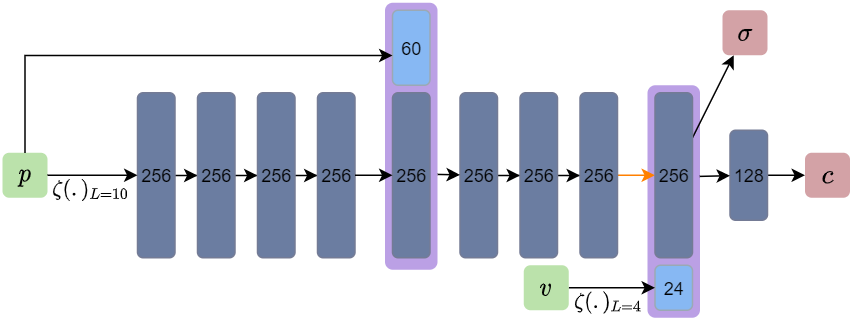
\includegraphics[width=0.6\textwidth]{figures/mlp_nerf.png}
    \caption{MLP used in NeRF \cite{mildenhall2020nerf} Dark blue boxes represent hidden layers. Black arrows indicate FC-layers with sigmoid activation, orange arrows - FC-layers without activation. $\zeta(.)$ stands for positional encoding function. $\sigma$ is 1D volume density, $c$ is a 3D color value. }
    \label{fig:mlp_nerf}
\end{figure}

\im{This paragraph should probably be moved to the related work.. somehow}
\cite{mildenhall2020nerf} propose to use a Multi-Layer Perceptron (MLP) as a representation
of an implicit function $F = F_\Theta$ with parameters $\Theta$.
The scheme structure of original NeRF's MLP is outlined in \Cref{fig:mlp_nerf}.
The position $p(z)$ is first encoded using position encoding function $\zeta(\cdot)$ (positional encoding is described in section \ref{subsec:pos_enc}) and then is processed with 8 fully-connected neural layers with ReLU activations.
The resulting feature vector is then concatenated with positionally encoded vector direction $v$
before the the volume density $\sigma(p(z))$ and the color value $c(p(z), v)$ is outputed.
The important concept here is that $\sigma$ only depends on point $p(z)$
whilst the color value $c$ is view dependant as well.
This setting is required to encourage the MLP to be multi-view consistent.

In order to perform the volume rendering, the continuous integral from equation \Cref{eq:rendering_equation} has to be solved.
One can estimate this integral using a discrete set of densely sampled points as proposed by \cite{mildenhall2020nerf}.
Separating each ray into $N$ bins and drawing random samples from each bin
makes the representation able to learn continuous function
while only using finite number of samples.
The estimate for the integral $C(p, v)$ will have a form (\cite{mildenhall2020nerf}, \cite{max1995optical}):

\begin{equation}
    \label{eq:integral_estimation}
    C(p, v) \approx \sum_{i=1}^{N} \tau_c(p_i) (1 - \exp (-\sigma(p_i) \delta_i)) c(p_i, v),
\end{equation}
where $p_i = p(z_i)$ for brevity, $\tau_c(p_i) = \exp (-\sum_{j=0}^i \sigma(p_j) \delta_j )$ is the accumulated transmittance and $\delta_i = z_{i+1} - z_i$ is the distance between adjacent sample points.

\subsection{Positional encoding}
\label{subsec:pos_enc}

Neural networks are known as a highly representative class of functions (\cite{hornik1989multilayer}).
However, recent works (\cite{rahaman2019spectral}, \cite{tancik2020fourfeat}) demonstrate the tendency of
biasing towards low frequency functions during training of deep neural networks.
The results can be smoothed and blurry as frequency-dependant learning speed
is much slower for high-frequency parts of the scene.
\cite{rahaman2019spectral} show that one can highly improve the quality of the MLP outputs
by using an embedding, which maps inputs to a higher dimensional space before passing them to the MLP.

The positional encoding function $\zeta(p) : \mathbb{R} \xrightarrow{} \mathbb{R}^{2L}$ as proposed by \cite{mildenhall2020nerf}, \cite{vaswani2017attention} is represented by Fourier series in the following form:

\begin{equation}
    \zeta(p) = (\sin(2^0\pi p), \cos(2^0\pi p), ..., \sin(2^{L-1}\pi p), \cos(2^{L-1}\pi p))
\end{equation}




\subsection{Sparse Voxels Octree}

The already described approach already is able to represent scenes with a high accuracy.
However, the very inefficient way of sampling points along rays
makes the training very slow and tough,
since the model has to be repeatedly evaluated on unimportant samples
of free space or occluded regions that do not make a worthwhile contribution to the finally rendered color value.

\im{\subsubsection{one paragraph for: hierarchical sampling}}
In the original approach \cite{mildenhall2020nerf} propose the hierarchical volume sampling algorithm (similar to \cite{levoy1990efficient}),
when another "coarse" neural network is used in order to roughly estimate volume densities along the ray.
This insight is then used to perform a more informed sampling of main ("fine") network.
The "coarse" network is being optimized along with the main network, which can be considered as an overhead.
However, taking into account the increase of training convergence the overall training gets more efficient.


\cite{liu2021neural} propose another framework
that is able to increase the efficiency of this method
and make the training time by up to an order of magnitude faster.
The main contribution is the usage of sparse voxel octrees (\cite{laine2011EfficientSV}) to divide space into voxels
that are efficiently used for training MLPs with shared parameters.

This approach requires a slight elaboration on the problem formulation.
Let the whole scene being fully contained in a set of $K$ sparse voxels: $\mathbb{V} = {V_1, ..., V_k}$.
The scene can then be represented as a set of voxel-bounded implicit functions
\begin{equation}
    F(p, v) = F_\Theta^i(g_i(p), \zeta(v)), \forall p \in V_i,
\end{equation}
where each function $F_\Theta^i$ is modelled with an MLP with shared parameters $\Theta$:
\begin{equation}
    F_\Theta^i: (g_i(p), \zeta(v)) \xrightarrow{} (c, \sigma), \forall p \in V_i
\end{equation}
Here $g_i(p)$ is the representation of $p$ that is defined as:
\begin{equation}
    g_i(p) = \zeta ( \chi ( \{\Tilde{g_i}(p_j^*)\}_{j=1}^8 ) ),
\end{equation}
where $\{p_j^*\}_{j=1}^8, p_j^* \in \mathbb{R}^3$ is the set of eight vertices of voxel $V_i$,
$\Tilde{g_i} \in \mathbb{R}^d$ represent the feature vectors that are stored for each vertex of voxel $V_i$,
$\chi(\cdot)$ stands for trilinear interpolation,
and $\zeta(\cdot)$ is a post-processing function,
which corresponds to positional encoding function explained in \ref{subsec:pos_enc}.

The volumetric rendering itself does not undergo any significant changes
except for some additional steps that have to be performed.
The sampling of the ray is only performed on the intervals of intersection with voxels $V_i$.
This allows to reject a descent amount of unimportant samples.
A very efficient Axis Aligned Bounding Box (AABB) ray intersection algorithm (\cite{haines1989essential}) is applied here
to extract the above mentioned intervals.
Another step is \textit{early termination}, which reduces the number of samples that have to be processed.
Since solid surfaces does not imply color values being dispersed along the ray,
the sample points that are behind the surface would be needless.
The technique here is to straight forwardly stop evaluating points,
that have an accumulated transmittance lower than some threshold.

The training on the scene begins with the octree,
which consists of $N$ voxels that fit in bounding box of the whole scene
and cover all parts of the scene.
One can get rid of non-essential voxels by performing a \textit{self-pruning} procedure.
This technique leverages the property of neural radiance fields
to extract some coarse scene geometry during early training iterations.
The decision if voxel is going to be pruned is made by uniformly sampling $G$ points inside the voxel
and comparing the minimum transmittance value with some threshold value $\gamma$ or more formally when:
\begin{equation}
    \underset{j=1 \dots G}{min} {\exp (- \sigma (g_i(p_j)))} > \gamma, p_j \in V_i, V_i \in \mathbb{V},
\end{equation}
where $\sigma (g_i(p_j))$ is the model prediction for $\sigma$ when processing $g_i(p_j)$.
The pruning procedure has to be performed regularly as the accuracy of the model increases as it gets more and more trained,
which means that more voxels can be pruned and therefore rejected from processing.

As model learns more detailed representation of the scene it becomes necessary to refine voxel structure.
During the refinement procedure each voxel is being subdivided into $2^3$ subvoxels by halving the voxel size.
Ray sampling steps are also being halved at this point in order to correspond new voxel size value.
The feature representation vectors $\Tilde{g_i}$ of the new vertices are initialized similarly to calculating $G_i(p)$,
namely using trilinear interpolation function $\chi(\cdot)$.
This scheme allows to achieve more detailed scene representation
and also increases the model capacity.



\subsection{Neural Reflectance Fields}

Although the neural radiance fields approach is able to produce realistic renderings under novel view conditions,
one of main limitations of this method is the inability to handle any kind of visual effects related to dynamic light conditions.
The core assumption of these approaches is a static illumination,
which is implicitly presented in the color values of the rendered images.
This in turn does not allow to change illumination on the rendering phase.

\cite{bi2020neural} propose the framework for eliminating this exact limitation.
Authors introduce neural reflectance field (NRF), which is the neural scene representation
that in addition to scene geometry also encodes normal and reflectance properties of the scene.
This approach allows to evaluate an explicit reflectance model at the selected point after all.
Although \cite{bi2020neural} focus on the microfacet bidirectional reflectance distribution function (BRDF) (\cite{walter2007microfacet}),
any other reflectance model can be used within this method as well
(i.e. authors also show some results of furry objects using hair reflectance model \cite{kajiya1989fur}).

This method uses the same rendering framework as proposed by \cite{mildenhall2020nerf}.
Assuming that the volume containing the scene to be only scattering volume (i.e. there are no emission or absorption processes),
the corresponding rendering equation \Cref{eq:rendering_equation} (\cite{Novak18volumeSTAR}) looks similarly
except for operating with radiance values $L$ instead of color values $c$:
\begin{equation}
    L(p, v) = \int_0^\infty \omega(p(z)) \cdot L_s(p(z), v) dz = \int_0^\infty \tau_c(p(z)) \sigma(p(z)) \cdot L_s(p(z), v)dz,
\end{equation}
where $L_s(p(z), v)$ denotes the scattered light at point $p(z)$ along direction $v$.

In general case $L_s$ is calculated by integrating incident radiance along the whole unit sphere $\mathbb{S}$:
\begin{equation}
    \label{eq:radiance_Li}
    L_s(p, v) = \int_\mathbb{S} f_p(p, v, l) L_i(p, l)dl,
\end{equation}
where $l$ is the 3D Cartesian representation of directions of the incident radiance $L_i(p, l)$.
$f_p(p, v, l)$ is the phase function, which controls
how the light that comes from $l$ scatters at point $p$ if viewing from $v$.

\cite{bi2020neural} only assume single light source setting
and the reflectance function as the phase function,
which allows to simplify \Cref{eq:radiance_Li}:
\begin{equation}
    L_s(p, v) = f_r(p, v, l, n(p), R(p)) L_i(p, l),
\end{equation}
where $f_r$ denotes a differentiable reflectance function
with parameters $R$.
Normal vector $n$ is also required for evaluation of reflectance model $f_r$.
$L_i(p, l)$ is the radiance that arrives from direction $l$ and can be calculated using light intensity $L_l(p)$
and the transmittance value $\tau_l(p, l)$,
which indicates the loss of light from the light source to the sample point $p$ along light ray $l$, as follows:
$L_i(p, l) = \tau_l(p, l) L_l(p, l)$.
The light attenuation coefficient $f_{att}$ is considered inside the $L_l$ term:
$L_l(p, l) = \frac{1}{d^2 / r^2}$,
where $d$ is distance from sample point $p$ to the light source
and $r$ is the light's radius (assuming light source to be an emissive sphere with radius $r$).

Combining these equations together and applying the same technique for numerical integral estimation
as used by \cite{mildenhall2020nerf} and \cite{liu2021neural} gives the following formulation of \Cref{eq:integral_estimation} for NRF:
\begin{equation}
    L(p, v, l) \approx \sum_{i=1}^N \tau_l(p_i, l) L_l(p_i, l) f_r(p_i, v, l, n(p_i), R(p_i)) \tau_c(p_i) (1 - \exp (-\sigma(p_i)\delta_i))
\end{equation}
Here $\tau_l$ plays the same role for light ray $l$
as $\tau_c$ operates for view ray $v$.
It is evaluated similarly along the light ray $l$:
$\tau_l(p_i, l) = \exp (-\sum_{j=1}^M \sigma(p'_j) \delta'_j)$,
where $p'(z') = p'_0 + z' \cdot l$ are sample points that are additionaly sampled along the light ray $l$ and $\delta'_j = z'_{j=1} - z'_j$.

This formulation covers the general case when light source can be located at arbitrary position.
Since the $l$ and $v$ vectors are different, the additional sampling of light ray is required,
which makes 


\section{Implicit Neural Reflectance Field}

Existing BRDF models limits the type of scenes that can be captured
and successfully reconstructed afterwards.
To model object appearance one can employ neural network, which is able to get trained for a very complex appearance representations.
In this work I \im{we?} call this technique as "Implicit scheme".

Texture predictor not only is dependant on view direction,
but also requires the light direction and distance to light source
(for modelling the light attenuation effect).
Figure \# shows the network structure for this approach.

\begin{enumerate}
    \item Light rays are not sampled (-> varying light transmittance either not considered or assumed to get learned by network\im{???})
    \item |--> Tangential space for coordinates (and parametrization as half-vectors. not done)
\end{enumerate}

Since the appearance effects happen mostly in a local coordinate frame, the usage of the global direction vectors implies on the model to learn global to local coordinate system transformation. Although this is generally achievable, the overall complexity of the task can be too overwhelming for the model and some kind of correlations might affect the model. In order to increase the training performance this transformation can be done deterministically and the view and light directions in local coordinate frame are to be passed to the input of the model.

The usage of the cartesian vectors is not very effective for reflectance representations. The half diff vectors (rusinkiewicz parametrization) can be used instead of positionally encoded l and v.
\sm{or in combination with positional encoding}




\section{Explicit Neural Reflectance Field \im{for arbitrary light source}}

The NRF inherits very poor performance behavior from NeRF,
which limits it to only be feasible for the co-located light source setting.
However, with some optimization techniques \cite{NSVF, ...} can be used to make this method practical.

Using Octree with Sparse Voxels \cite{NSVF} highly increases the efficiency of sampling view rays,
and using voxel features allows to use smaller networks,
which also speeds up the training.

This efficiency improvement makes the general problem statement with an arbitrary light source feasible.


\section{In-Voxel Approximation}

Using the octree allows to approximate light rays sampling inside voxels in order to increase the performance of the method.

Instead of performing inverse CDF sampling as it is done for view rays, one can do the following:
\begin{enumerate}
    \item Bravely \sm{colloquial} assume the media homogenious inside voxels and boldly approximate it as constant
    \item Under the same brave assumption perform some sampling inside the voxel once at N iterations (e.g. right after pruning has been performed)
    \item The in-voxel sampling can be lighter than inverse CDF (e.g. just sample the center of voxel, or voxel corners + trilinear interpolation)
\end{enumerate}


% NSVF proposed a good technique of using Sparse Voxel Trees in order to increase the rendering speed. However, the scene is still lacking the light interaction.

% One can achieve this by also passing light directions along with distance to the light source into the network, in order to make it distinguish different surface properties for different view and light directions.








% This is some test area for new mathematical helper macros to nicely visualize mathematical formulas.

% \section{Numbers}
% \begin{align}
%     \mathbb{C}
%     \qquad
%     \mathbb{R}
%     \qquad
%     \mathbb{Q}
%     \qquad
%     \mathbb{Z}
%     \qquad
%     \mathbb{N}
% \end{align}

% \section{Numbers with physical units}
% \begin{align}
%     \SI{1.23}{\meter\per\second}
% \end{align}
% \begin{align}
%     \si{\meter\per\second}
% \end{align}
% \begin{align}
%     \SI{1.23\pm0.45}{\meter\per\second}
% \end{align}
% \begin{align}
%     \SI{3e8}{\meter\per\second}
% \end{align}
% \begin{align}
%     \SI{32}{\giga\byte} = \SI{32e9}{\byte}
% \end{align}
% \begin{align}
%     \SI{32}{\gibi\byte} = \SI[exponent-base=2]{32e30}{\byte}
% \end{align}

% \section{Norm, Dot, Abs, Interval}
% \begin{align}
%     \pi = \const
% \end{align}
% \begin{align}
%     1 \in \interval{0}{2}
% \end{align}
% \begin{align}
%     1 \in \order{n}
% \end{align}
% \begin{align}
%     \evalat{ \frac{\partial f}{\partial x} }{ x = 0 }
% \end{align}
% \begin{align}
%     \norm{p} \qquad \norm{\frac{p}{2}}
% \end{align}
% \begin{align}
%     \abs{p} \qquad \abs{\frac{p}{2}}
% \end{align}
% \begin{align}
%     \dotproduct{p}{q} \qquad \dotproduct{\frac{p}{2}}{q}
% \end{align}
% \begin{align}
%     \crossproduct{p}{q} \qquad \crossproduct{\frac{p}{2}}{q}
% \end{align}

% \section{Vector, Matrix}
% \begin{align}
%     \vec{p} \qquad \vecarrow{p}
% \end{align}
% \begin{align}
%     \vec{p}^{\transposed}
% \end{align}
% \begin{align}
%     \gradient{\vec{p}}
% \end{align}
% \begin{align}
%     \divergence{\mat{A}}
% \end{align}
% \begin{align}
%     \laplacian{\mat{A}}
% \end{align}
% \begin{align}
%     \mat{A}
% \end{align}
% \begin{align}
%     \set{K} , K
%     \qquad
%     \set{N} , N
% \end{align}
% \begin{align}
%     \neighborhood{\vec{p}} = \left\{ \vec{q} \mid \norm{\vec{p} - \vec{q}} < \epsilon \right\}
% \end{align}

% \section{Set operations}
% \begin{align}
%     A \intersect B
% \end{align}
% \begin{align}
%     A \union B
% \end{align}
% \begin{align}
%     A \difference B
% \end{align}

% \section{Derivative, Integral, Sum, Probability}
% \begin{align}
%     \int_H x \, dx
% \end{align}
% \begin{align}
%     \sum_H x
% \end{align}
% \begin{align}
%     \probability{x}
% \end{align}
% \begin{align}
%     \probabilitygiven{x}{y}
% \end{align}
% \begin{align}
%     \expectation{x}
% \end{align}
% \begin{align}
%     \deviation{x}
% \end{align}
% \begin{align}
%     \variance{x}
% \end{align}


% \section{Lemma, Theorem, Corollary}
% \begin{lemma}
%     This is a lemma.
% \end{lemma}
% \begin{proof}
%     Proof of lemma.
% \end{proof}

% \begin{theorem}
%     This is a theorem.
% \end{theorem}
% \begin{proof}
%     Proof of theorem.
% \end{proof}

% \begin{corollary}
%     This is a corollary.
% \end{corollary}
% \begin{proof}
%     Proof of corollary.
% \end{proof}


